\documentclass[Orbiter User Manual.tex]{subfiles} 
\begin{document}

\section{Included spacecraft types}
Orbiter comes with a range of diverse spacecraft types to explore different aspects of space flight. This includes fictional spacecraft such as the Delta-glider and Shuttle-A which relax a few specifications beyond current limits (in particular in terms of fuel efficiency and structural strength) to allow flights across the solar system, recreations of real vessels such as the Space Shuttle with narrow error margins that require precise flight plans, to novel concepts such as solar sails.\\
The spacecraft included in the basic Orbiter distribution will get you started, but many more can be downloaded as add-ons. See the Orbiter web page for a list of add-on repositories.


\subsection{Delta-glider}
% TODO


\subsection{Shuttle-A}
% TODO


\subsection{Shuttle PB (PTV)}
The PB is a very agile single-seat spacecraft. It has a main engine and uses hover thrusters for vertical take-off and landing. During atmospheric flight the lifting body and winglets produces lift. However, aerodynamic control surfaces are not supported in the current version. Attitude control is performed via the reaction control system (RCS).\\

\begin{figure}[H]
  \centering
  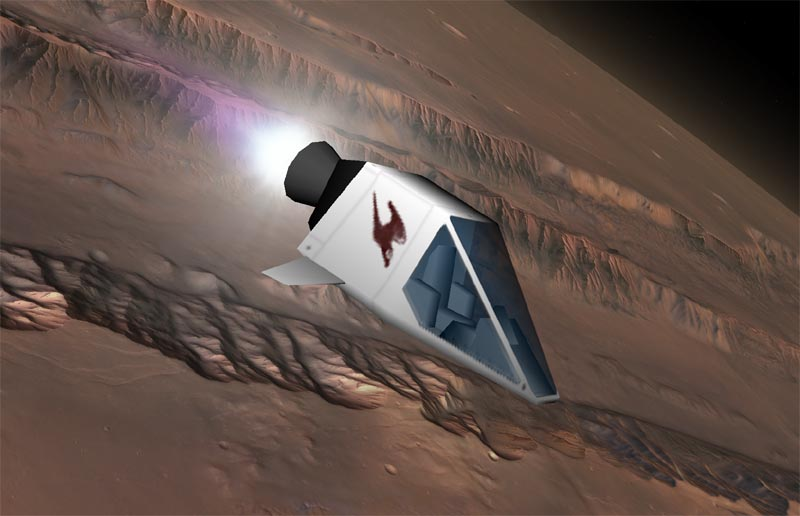
\includegraphics[width=0.75\hsize]{shuttle_pb.jpg}
  \caption{Overall design and textures: Balázs Patyi. Model improvements: Martin Schweiger}
\end{figure}

\noindent
%TODO add section link
Apart from the standard implementation of the PB vessel class, Orbiter also comes with a script version of this spacecraft type (\textit{ScriptPB}). This looks and behaves identical to the original Shuttle PB, but is completely implemented as a Lua script (see chapter TODO) and can therefore easily be modified. This is a good way for newcomers to get into spacecraft design. The code can be found in Config\textbackslash ScriptPB.cfg.\\
\\
\textbf{Technical specifications:}

%\begin{table}[H]
	%\centering
	\begin{longtable}{ |p{0.25\textwidth}|p{0.15\textwidth}|p{0.05\textwidth}|p{0.45\textwidth}| }
	\hline\rule{0pt}{2ex}
	Mass & 500 & kg & (empty)\\
	\hline\rule{0pt}{2ex}
	& 750 & kg & (fuel capacity)\\
	\hline\rule{0pt}{2ex}
	& 1250 & kg & (total)\\
	\hline\rule{0pt}{2ex}
	Dimensions & 6.8 x 5.2 x 2.4 & m & (L x W x H)\\
	\hline\rule{0pt}{2ex}
	Thrust & 30.0 & kN & (main)\\
	\hline\rule{0pt}{2ex}
	& 2 x 7.5 & kN & (hover)\\
	\hline\rule{0pt}{2ex}
	Acceleration & 24.0 & m/s$^{2}$ & (main thrust at full load)\\
	\hline\rule{0pt}{2ex}
	Isp & 5.0 $\cdot$ 10$^{4}$ & m/s & (vacuum)\\
	\hline
	\end{longtable}
%\end{table}



\subsection{Dragonfly}
% TODO


\subsection{Space Shuttle Atlantis}
% TODO


\subsection{International Space Station (ISS)}
The International Space Station is a multinational scientific orbital platform in low Earth orbit (orbital altitude $\sim$420 km). It is composed of multiple modules that were assembled in orbit from 1998. It has been continuously occupied since 2000 and is expected to be in operation until 2030. Many of the assembly missions (with the exception of the Russian modules) and crew operation missions were flown by the Space Shuttle until its retirement in 2011, which makes the ISS a good mission target for your Shuttle flights. Docking the Space Shuttle manually at the ISS with its Orbital Docking System installed in the payload bay is a challenge even for experienced pilots.

\begin{figure}[H]
  \centering
  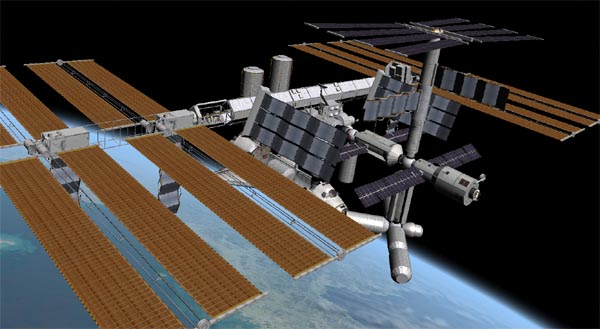
\includegraphics[width=0.75\hsize]{iss.jpg}
  \caption{3D model and textures: Project Alpha by Andrew Farnaby}
\end{figure}

\noindent
The ISS is equipped with multiple docking ports. In Orbiter, they are outfitted with IDS (Instrument Docking System) transmitters to feed the onboard docking instruments. The default IDS frequencies are listed in the table.

%\begin{table}[H]
	%\centering
	\begin{longtable}{ |p{0.1\textwidth}|p{0.15\textwidth}| }
	\hline\rule{0pt}{2ex}
	Port 1 & 137.40  MHz\\
	\hline\rule{0pt}{2ex}
	Port 2 & 137.30  MHz\\
	\hline\rule{0pt}{2ex}
	Port 3 & 137.20  MHz\\
	\hline\rule{0pt}{2ex}
	Port 4 & 137.10  MHz\\
	\hline\rule{0pt}{2ex}
	Port 5 & 137.00  MHz\\
	\hline
	\end{longtable}
%\end{table}

\noindent
In addition, a transponder (XPDR) for long-range tracking at frequency 131.30 MHz is equipped.

\begin{figure}[H]
  \centering
  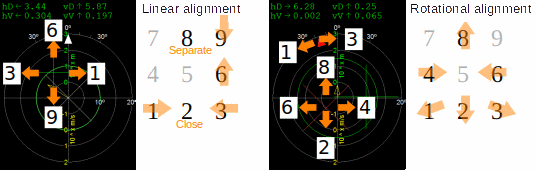
\includegraphics[width=0.75\hsize]{iss_dock.png}
  \caption{Effect of RCS command input on linear/rotational alignment cues in Docking MFD for Shuttle with docking adapter installed in cargo bay.}
\end{figure}


\subsection{Space Station Mir}
Mir was a Soviet (later Russian) modular space station in low Earth orbit ($\sim$360 km altitude) between 1986 and 2001. It was assembled in stages, with modules delivered to orbit mostly by Proton rockets. It was the largest man-made object in orbit before being surpassed by the ISS. It was continuously inhabited and still holds the record for longest human spaceflight. At the end of it service life it was de-orbited and burnt up in the atmosphere, with remaining fragments falling into the South Pacific Ocean.\\

\begin{figure}[H]
  \centering
  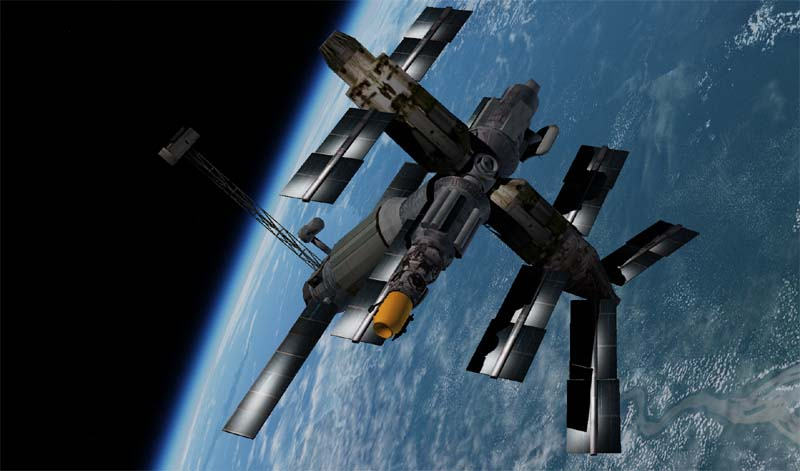
\includegraphics[width=0.75\hsize]{mir.jpg}
  \caption{Mir model and textures by Jason Benson.}
\end{figure}

\noindent
In Orbiter, Mir is still in orbit and can be used for rendezvous and docking manoeuvres. Unlike its real-life counterpart, it is orbiting in the plane of the ecliptic, which makes it a good staging platform for translunar and interplanetary missions.\\
Mir supports 3 docking ports, which in Orbiter are equipped with IDS with transmitting at the frequencies listed in the table. It also has a long-range transponder (XPDR) at 132.10 MHz.

%\begin{table}[H]
	%\centering
	\begin{longtable}{ |p{0.1\textwidth}|p{0.15\textwidth}| }
	\hline\rule{0pt}{2ex}
	Port 1 & 135.00  MHz\\
	\hline\rule{0pt}{2ex}
	Port 2 & 135.10  MHz\\
	\hline\rule{0pt}{2ex}
	Port 3 & 135.20  MHz\\
	\hline
	\end{longtable}
%\end{table}


\subsection{Lunar Wheel Station}
This is a large fictional space station in orbit around the Moon. It consists of a wheel, attached to a central hub with two spokes. The wheel has a diameter of 500 m and is spinning at a frequency of one cycle per 36 s, providing its occupants with a centrifugal acceleration of 7.6 m/s$^{2}$, or about 0.8 g, to mimic Earth's surface gravitational force.

\begin{figure}[H]
  \centering
  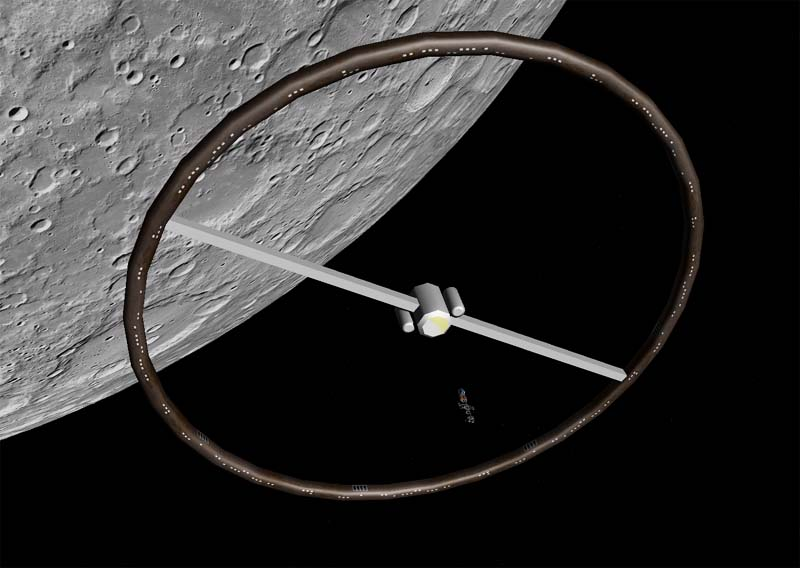
\includegraphics[width=0.75\hsize]{lunar_wheel.jpg}
  \caption{A Shuttle-A on final approach to the Lunar Wheel station. Wheel model and textures: Martin Schweiger.}
\end{figure}

\noindent
%TODO add section link
The main problem the station poses to an approaching spacecraft is the rotational alignment in preparation for docking. Docking with a rotating target is only possible along the rotation axis. The station has two docking ports in the central hub, with approach directions along the axis from either side. Before docking, the approaching vessel must synchronise its own rotation around its longitudinal axis with that of the station. This should happen as late as possible (within 10 m separation), because corrections in the lateral position become very difficult once the spacecraft is rotating. For docking procedures, see Chapter TODO.\\

\alertbox{Currently, Orbiter's docking alignment instrumentation works with rotating docking targets only if the ship's docking port is aligned with its longitudinal axis of rotation. This is the case for Shuttle-A and Dragonfly, but not for the Delta-glider. And should you somehow get the Space Shuttle into a lunar orbit, don't even try to dock at the Wheel.}

\noindent
\\
The Wheel station emits a transponder signal at frequency 132.70 MHz. The default IDS transmitter frequencies for the two docking ports are listed in the table.

%\begin{table}[H]
	%\centering
	\begin{longtable}{ |p{0.1\textwidth}|p{0.15\textwidth}| }
	\hline\rule{0pt}{2ex}
	Port 1 & 136.00  MHz\\
	\hline\rule{0pt}{2ex}
	Port 2 & 136.20  MHz\\
	\hline
	\end{longtable}
%\end{table}


\subsection{Hubble Space Telescope}
The Hubble Space Telescope (HST) was launched into low Earth orbit by Space Shuttle Discovery during mission STS-31 in 1990 and is still in operation as of 2022. Several on-orbit service missions have been carried out until the retirement of the Space Shuttle program, one of which was to install corrective optics to compensate for a shape error of the primary mirror which was discovered after the telescope had been launched.

\begin{figure}[H]
  \centering
  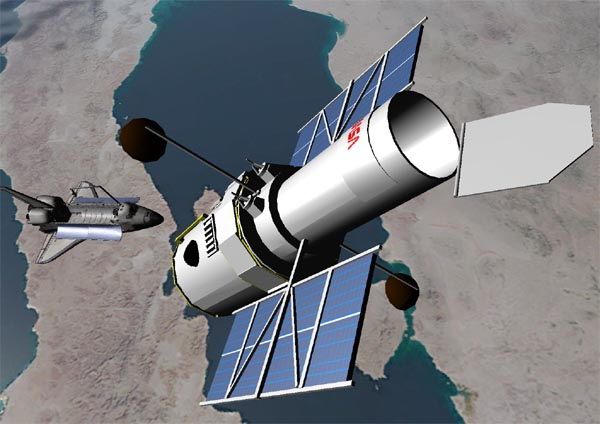
\includegraphics[width=0.75\hsize]{hst.jpg}
  \caption{HST model and textures by David Sundstrom.}
\end{figure}

\noindent
Hubble mainly operates in the visible frequency range (from near-infrared to ultraviolet). As a space-based telescope, it avoids image degradation from atmospheric effects, and during its long service life it provided images of unprecedented quality that significantly contributed to advance our understanding of the universe. Its observations range from solar system objects and events, such as the impact of comet Shoemaker-Levy on Jupiter, to deep-field images of the faintest and most distant objects yet observed in the visible band. Notable discoveries to which Hubble data contributed include the accelerated expansion of the universe, the prevalence of supermassive black holes in the centres of galaxies, detection of exosolar planets and evidence of star formation.\\
%TODO add section link
Orbiter provides several Space Shuttle\textbackslash HST missions for both deployment and recapture operations. For Shuttle payload manipulation, see Chapter TODO.\\
\\
\textbf{Vessel-specific key controls:}

%\begin{table}[H]
	%\centering
	\begin{longtable}{ |p{0.2\textwidth}|p{0.7\textwidth}| }
	\hline\rule{0pt}{2ex}
	\textbf{Shortcut} & \textbf{Action}\\
	\hline\rule{0pt}{2ex}
	1 & Deploy/retract high-gain antennae\\
	\hline\rule{0pt}{2ex}
	2 & Open/close telescope tube hatch\\
	\hline\rule{0pt}{2ex}
	3 & Deploy/fold solar arrays\\
	\hline
	\end{longtable}
%\end{table}


\subsection{LDEF Satellite}
The Long Duration Exposure Facility (LDEF) was an orbital platform designed to provide experimental data on the effect of space environment on materials, biological samples and operational procedures. It was delivered to orbit by Space Shuttle Challenger in 1984 (mission STS-41 C). It was intended to be recaptured and returned to Earth a year later, but due to delays in the aftermath of the Challenger accident, was stranded in space for six years and eventually recovered from its decaying orbit on January 11, 1990 by Columbia (STS-32), two months before it would have burnt up in the atmosphere.

\begin{figure}[H]
  \centering
  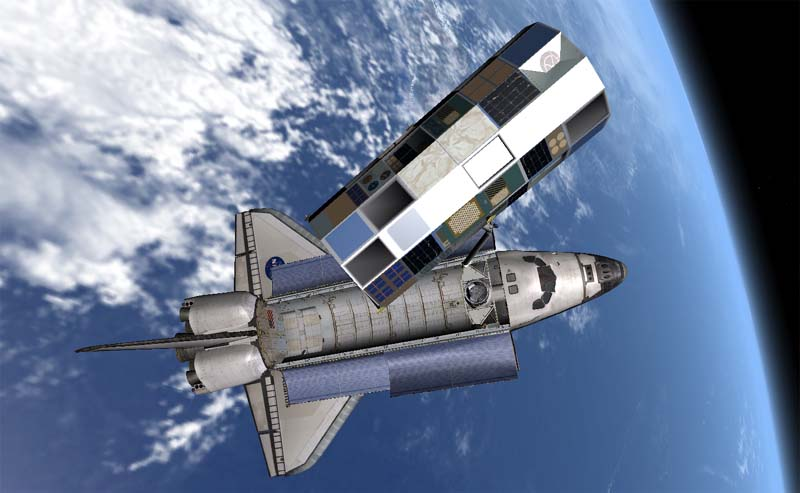
\includegraphics[width=0.75\hsize]{ldef.jpg}
  \caption{LDEF mesh by Don Gallagher.}
\end{figure}

\noindent
The LDEF makes a good object for Shuttle deployment and retrieval missions in Orbiter. Scenario folder Satellites and Probes\textbackslash LDEF contains missions for LDEF operations.


\end{document}
